
%(BEGIN_QUESTION)
% Copyright 2012, Tony R. Kuphaldt, released under the Creative Commons Attribution License (v 1.0)
% This means you may do almost anything with this work of mine, so long as you give me proper credit

Determine the amount of air pressure applied to this piezoresistive pressure sensor, assuming the sensor has a linear response to pressure (1 k$\Omega$ at 0 PSI, 2 k$\Omega$ at 5 PSI, 3 k$\Omega$ at 10 PSI, 4 k$\Omega$ at 15 PSI) and the output voltage signal is 1.3 volts:

$$\includegraphics[width=15.5cm]{i03537x01.eps}$$

$P$ = \underbar{\hskip 50pt} PSI

\vskip 10pt

Also, determine if the signal voltage will {\it increase} or {\it decrease} as pressure increases.

\underbar{file i03537}
%(END_QUESTION)





%(BEGIN_ANSWER)

\noindent
Half credit for each answer:

\vskip 10pt

$P$ = \underbar{\bf 3.885} PSI

\vskip 10pt

(Deduct 3 points if the answer was derived graphically rather than analytically)

\vskip 10pt

The signal voltage will {\bf decrease} as applied pressure increases.


%(END_ANSWER)





%(BEGIN_NOTES)

{\bf This question is intended for exams only and not worksheets!}.

%(END_NOTES)


